\section{\instType{} Client Software}
\label{sec:Software}

The \instType{}-pH requires the use of its own client software for programming, download and data interpretation.


\subsection{\instType{} Client Installation}
\label{sec:Install}

\instType{} software is available for both Windows (XP and later) and Mac (OS X).  To install the software, simply insert the \instType{} Software disc, navigate to the \textbf{SAMI\_Client Application} folder and drag the folder for your computer platform to an appropriate location on your hard drive.  You may want to create a shortcut to your application, but it is important that the application itself remain in the folder with the various sub-folders and other files for it to operate correctly.  When you open the \instType{} Client, if connected to the internet, the software will automatically search for updates.  You can update your software at \url{http://www.sunburstsensors.com/swupdate}


\subsubsection{USB Serial Driver}

Also on the disc is the driver for the serial-USB converter that is part of your communication cable. Most modern computers will already have appropriate drivers installed or automatically install this driver from the internet.  If your computer does not recognize the USB-serial converter when the cable is plugged in, you can opt to install from this folder.  You may also use the internet to download the latest driver from \url{http://ftdichip.com/Drivers/VCP.htm}


\subsubsection{\instType{} Cables and Bulkheads}
\label{Cable}

\ifcase \inst	%iSAMI

The black communication cable included with your instrument will have a 6-pin bulkhead connector on one end and on the other end, two diverging cables: a USB and banana plugs. 

The black (ground) and red (positive) banana plugs should be connected to a DC power supply set to 10--13\,VDC. The USB connects directly to one of your computer's USB ports.

The \instType{} uses wet-pluggable bulkhead connections made by Impulse or SubConn.  To communicate with the \instType{}, remove the bulkhead cover plug by unscrewing the locking collar and pulling firmly up. Take care to not unscrew the bulkhead itself, which requires adequate torque (15\,in-lb or 1.7\,Nm) to maintain its seal. To connect the communication/power cable, align the pins on the cable with the receptacles on the \instType{} bulkhead and push down firmly.

The \instType{} uses the RS-232 communication protocol. Figure \ref{fig:Subconn} shows the pin-out of the bulkhead as you look down on it.

The Tx line transmits data out and while the Rx line is how commands are sent to the unit. The RTS line tells the \instType{} that it is connected to the client software. While it is held high the \instType{} will send out status strings about once per second. If connecting to a terminal, or external logger, keep RTS off.  RTS on the client software expires after three minutes to save power (See section \ref{sec:Software}).

    \textbf{The \instType{} internal battery has enough power to maintain the datalogger for about 90 days. Once the internal batteries die, your \instType{} will not be able to store data.} Therefore, the recommended sequence for storing, programming, powering, and running, the \instType{} is:
    
    \begin{enumerate}
    \item[]\textbf{\instType{} storage}. When storing the \instType{}, it should be left connected to a 12\,V battery pack or 12\,VDC power, in order to avoid draining the internal battery.
    
    \item[]\textbf{Running the \instType{} in the lab.} When running the \instType{} in the lab, it must be connected to 12\,VDC power.  The \instType{} will shut down if you attempt to run the pumps or a pH measurement using the internal batteries.
    
    \item[]\textbf{Programming the \instType{} for deployment.} The \instType{} can be programmed while connected to a computer, without external power.
    
    \item[]\textbf{Deploying the \instType{}.} The \instType{} must be connected to a 12\,V submersible battery pack or a 12\,VDC power supply during deployment.  The \instType{} will shut down when the 12\,V supply is removed.
    
    \item[]\textbf{Downloading data from the \instType{} after deployment.} Data can be downloaded from the \instType{} by disconnecting the 12\,V power and connecting the \instType{} to a computer.
    \end{enumerate}

\begin{figure}[t]
\centering
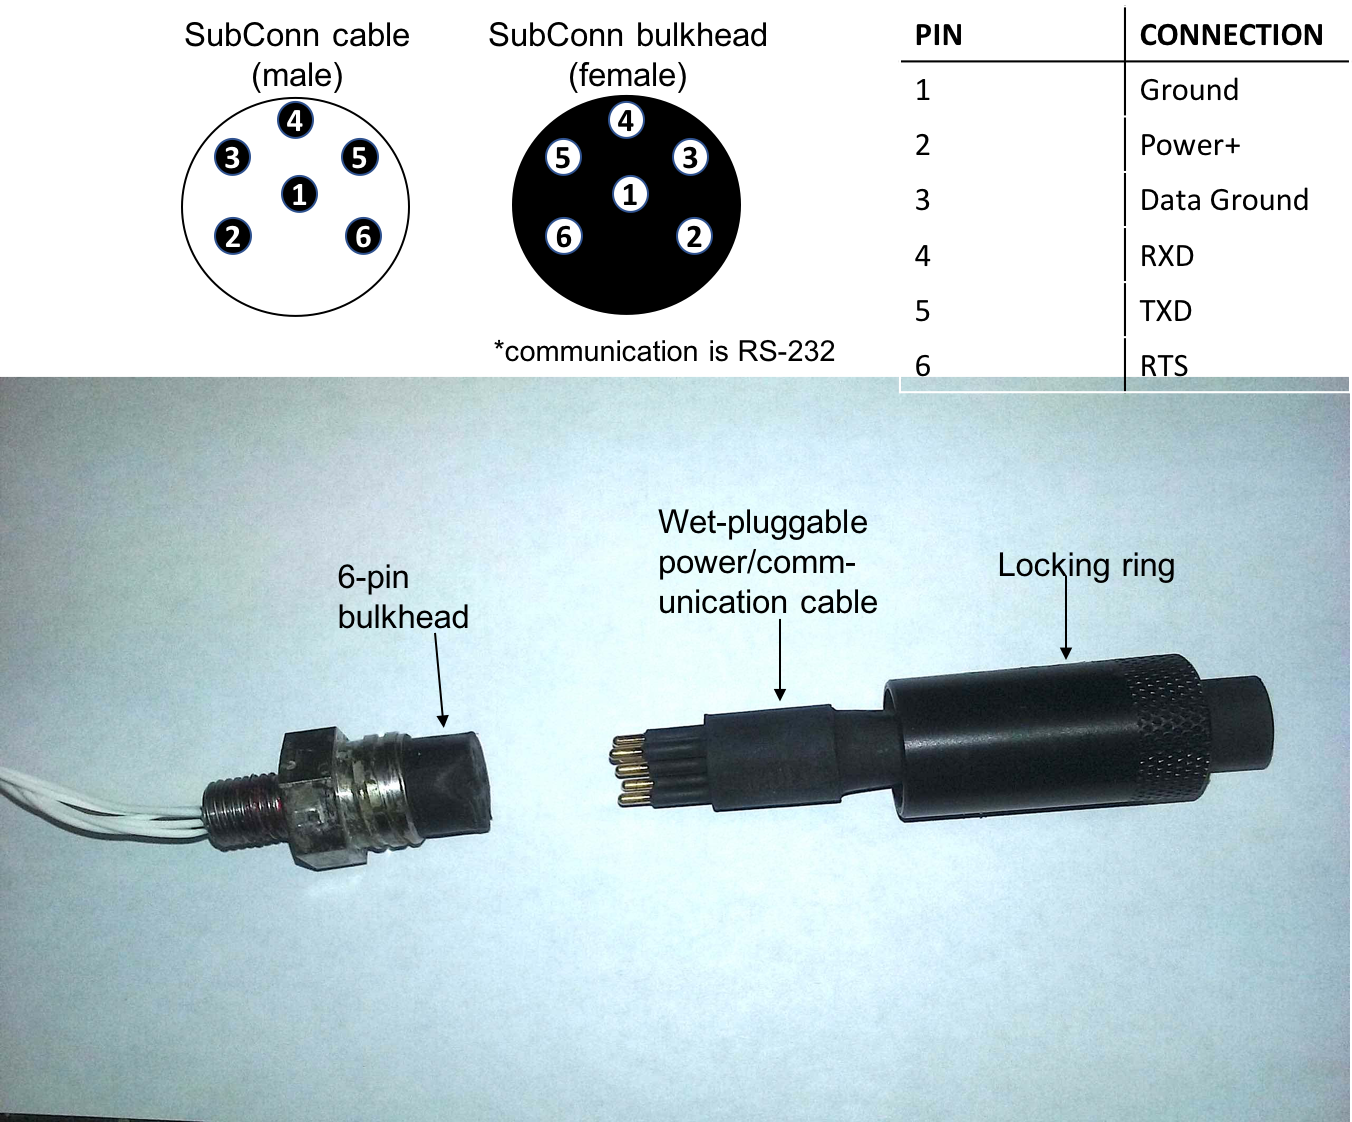
\includegraphics[width=0.8\textwidth]{figs/Subconn_cable.png}
\caption{\instType{} 6-pin connection.}
\label{fig:Subconn}
\end{figure}

\or		%SAMI

The black communication cable included with your instrument will have a 6-pin bulkhead connector on one end and on the other end, two diverging cables: a USB and banana plugs. 

The black (ground) and red (positive) banana plugs should be connected to a DC power supply set to 10--13\,VDC. If the voltage of the power supply is set to be greater than the voltage of the internal batteries, battery power can be saved. The USB connects directly to one of your computer's USB ports.

The \instType{} uses wet-pluggable bulkhead connections made by Impulse or SubConn.  To communicate with the \instType{}, remove the bulkhead cover plug by unscrewing the locking collar and pulling firmly up. Take care to not unscrew the bulkhead itself, which requires adequate torque (15\,in-lb or 1.7\,Nm) to maintain its seal. To connect the communication/power cable, align the pins on the cable with the receptacles on the \instType{} bulkhead and push down firmly. Before deploying the \instType{} be sure to replace the bulkhead cover pug and screw down the locking sleeve to protect the bulkhead pins from corrosion.

The \instType{} uses the RS-232 communication protocol. Figure \ref{fig:Subconn} shows the pin-out of the bulkhead as you look down on it.

The Tx line transmits data out and while the Rx line is how commands are sent to the unit. The RTS line tells the \instType{} that it is connected to the client software. While it is held high the \instType{} will send out status strings about once per second. If connecting to a terminal, or external logger, keep RTS off.  RTS on the client software expires after three minutes to save power (See section \ref{sec:Software}).

\begin{figure}[t]
\centering
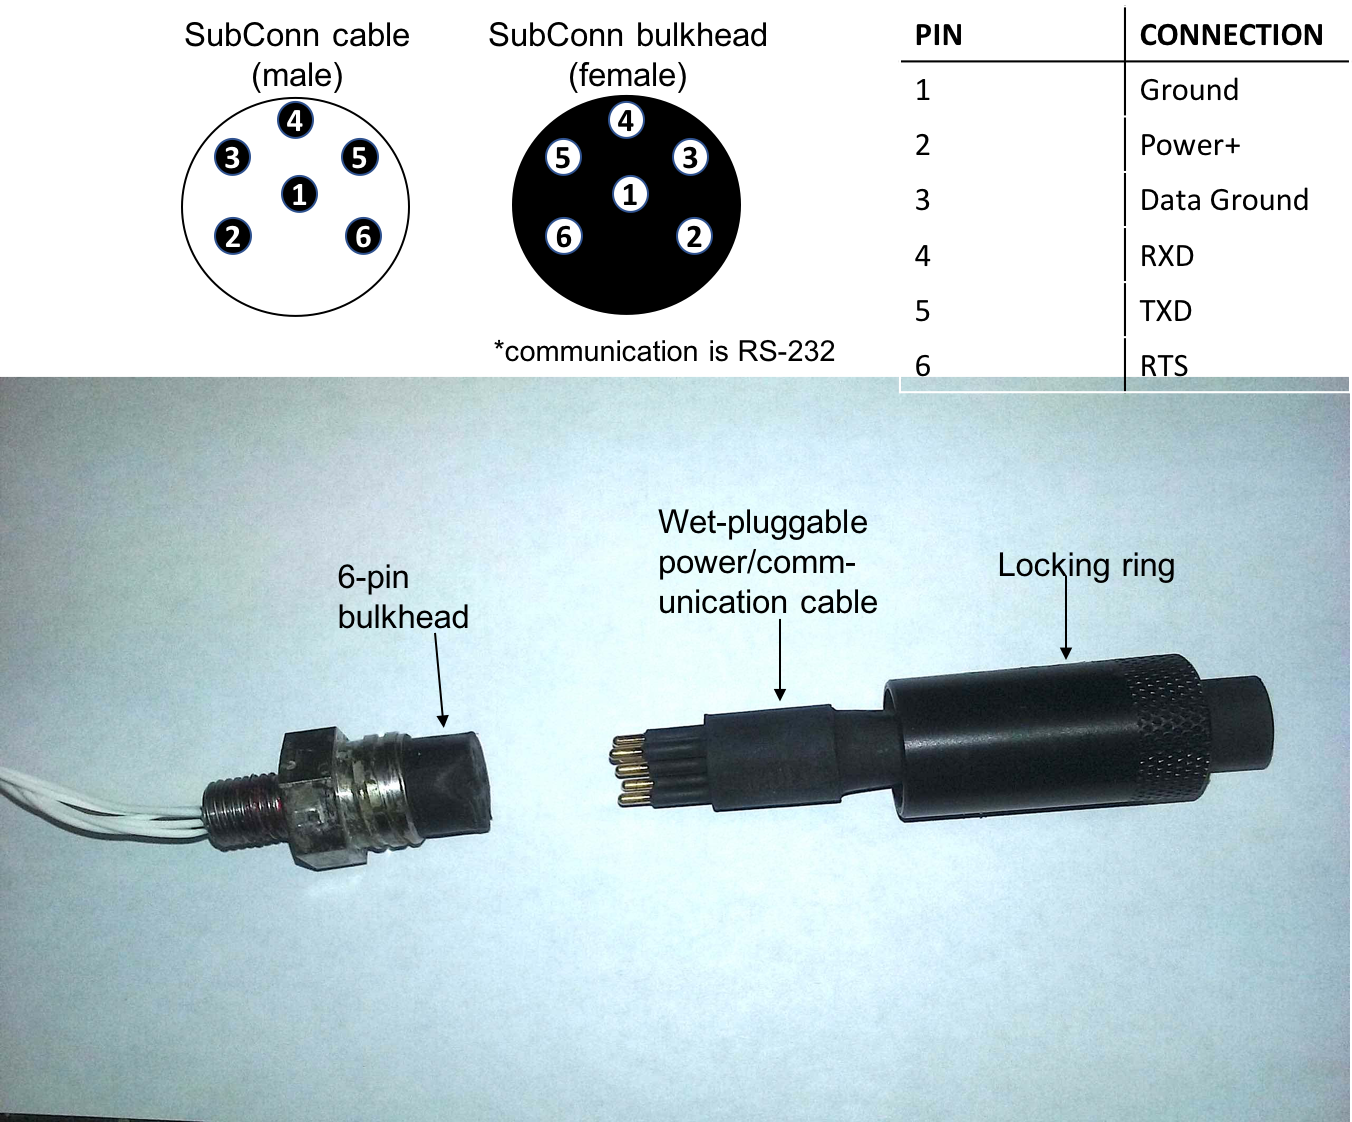
\includegraphics[width=0.8\textwidth]{figs/Subconn_cable.png}
\caption{\instType{} 6-pin connection.}
\label{fig:Subconn}
\end{figure}

\or		%AFT

The black communication cable included with your instrument will have a 6-pin connector on one end and on the other end, two diverging cables: a USB-serial converter and an AC power plug. The communication cable's bulkhead attachment should be attached to the side of your AFT instrument.  

\begin{table}[ht]
\RawFloats
\begin{minipage}[b]{0.5\hsize}
\centering
   \begin{tabular}{l l}
       \toprule
       Pin & Connection \\
       \midrule
       1 & DTR \\
       2 & RXD \\   
       3 & TXD \\
       4 & Signal GND \\
       5 & Power + \\
       6 & Power GND \\
       \bottomrule
    \end{tabular}
    \caption{Cable pin assigments.}
    \label{tab:BulginPins}
\end{minipage}
\hfill
\begin{minipage}[b]{0.5\hsize}
\centering
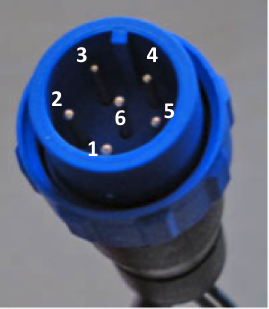
\includegraphics[scale=0.5]{figs/Bulgin_labeled.png}
\captionof{figure}{Bulgin cable connector.}
\label{fig:BulginCable}
\end{minipage}
\end{table}

\fi


\subsubsection{Communicating}

Once your instrument and computer are properly interfaced, you may start communicating with the instrument. Under \textbf{Preferences} (in the \textbf{Edit} menu for PCs, and in the \textbf{SAMI Client} menu for Macs) select the appropriate serial port. Click the \textbf{Serial Open} button to establish communication with your \instType{}. The indicator next to the Serial Port text will specify if your \instType{} is interfaced with your computer (Figure \ref{fig:InstInterface}). A red dot indicates a closed serial port while a green dot indicates an open serial port. 

Failure to connect usually indicates that the wrong port has been selected. Double check your port settings if you cannot connect. See also the troubleshooting section.

\begin{figure}[ht]
\centering
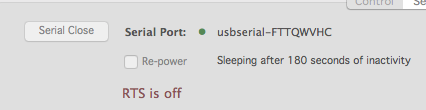
\includegraphics[width=0.6\textwidth]{figs/Inst_Interface.png}
\caption{Instrument interface.}
\label{fig:InstInterface}
\end{figure}


\subsection{Quick Start Guide}

The following procedure will guide you through the process of starting and stopping your \instType{}. A more detailed discussion can be found later in the user manual.  Please review the following checklist to ensure that the instrument is ready to start and deploy:

\begin{enumerate}
\item None of the housing compartments of your instrument have been opened since receipt. Sunburst cannot be held responsible for issues experienced if the instrument has been opened.
\item The instrument is being deployed within 90 days of receipt

\ifcase \inst	%iSAMI

\item Pump DI (deionized water in the attached bag) 30 times and check to see if liquid is coming out of the outlet tubing.
\item Remove DI Bag from inlet tubing.
\item If the instrument will be deployed through ice, remove copper bells from inlet tubing.

\or			%SAMI

\item Pump DI (deionized water in the attached bag) 30 times and check to see if liquid is coming out of the outlet tubing.
\item Remove DI Bag from inlet tubing.
\item If the instrument will be deployed through ice, remove copper bells from inlet tubing.

\or			%AFT

\fi

\item The instrument was not stored in freezing temperatures, in direct sunlight, or at high temperatures for extended periods of time.
\item If any of these points listed above were not met or if the instrument is not functioning properly prior to deployment, contact Sunburst Technical Support (techsupport@sunburstsensors.com).  Do NOT deploy instrument.
\end{enumerate}


\subsubsection{\instType{} Launch Procedure}

\begin{enumerate}

\ifcase \inst	%iSAMI

    \item Attach communication cable to \instType{}, power supply, and computer. Please note that the cable provided with the \instType{} is for bench-top programming and download of the \instType{} data.  The cable is not made for deployment, but can be used for shallow laboratory testing.
    
        \begin{enumerate}
        \item Attach the cable to the 6-pin bulk-head connection on the top of the \instType{}.
        \item Attach the banana plugs (black is ground, red is positive) to a +\,12\,VDC power supply.

        \textit{The \instType{} can be programmed for deployment in the field without a 12\,V power supply by connecting the cable to the bulkhead and to the computer.  However, the \instType{} must be connected to a 12\,V power supply \textbf{before} it begins measurements. Operation of the pump without a power supply will shut down the \instType{}.}
        
        \item Attach the USB connector to a USB port on your computer.
        \end{enumerate}
        
\or			%SAMI

    \item Attach communication cable to \instType{}, power supply, and computer. Please note that the cable provided with the \instType{} is for bench-top programming and download of the \instType{} data.  The cable is not made for deployment, but can be used for shallow laboratory testing.
    
        \begin{enumerate}
        \item Attach the cable to the 6-pin bulk-head connection on the top of the \instType{}.
        \item Attach the banana plugs (black is ground, red is positive) to a +\,12\,VDC power supply.
        \item Attach the USB connector to a USB port on your computer.
        \end{enumerate}
        
\or			%AFT

    \item Attach communication cable to \instType{}, power supply, and computer.
    
\fi    
    
    \item Install \instType{} Client software and the USB serial converter driver as described in section \ref{sec:Install}.
    
    \item The first time you run \instType{} Client, a preferences window should open allowing you to select the proper COM port.  The correct port will usually be the last one in the list on a Windows machine.  On a Mac the correct port will be \verb|usb serial Fxxxxxx| where ``x'' represents any alphanumeric character.
    
    \item If you want the application to automatically connect to the \instType{} using the same port in the future, check the box in preferences.  Dismiss the preferences dialog by clicking \textbf{OK}.
    
    \item If you did not check the box in step 4, click on the \textbf{Serial Open} button on the Control page.
    
    \ifcase \inst	%iSAMI
    
        \item Under the \textbf{Settings} tab, in the \textbf{SAMI} subpanel, choose SAMI pH (Vb+) from the dropdown menu.  \textbf{Set the desired \instType{} start time to a time at which the \instType{} will be connected to a 12\,V power supply or submersible battery pack.}  You may choose to record battery and temperature prior to start using the \textbf{Prestart} sub-panel.
        
    \else		%SAMI/AFT
    
        \item Under the \textbf{Settings} tab, in the \textbf{SAMI} subpanel, choose SAMI pH (Vb+) from the dropdown menu.  Set the desired \instType{} start time.  You may choose to record battery and temperature prior to start using the \textbf{Prestart} sub-panel.  If you have any external instruments they will be programmed using \textbf{Device 1, 2 or 3}.

    \fi
    
    \item Under the \textbf{Control} tab, click \textbf{Re-power} if Deployment Cycle Controls are not active.  Erase any data stored in the memory (download if desired), Launch!
    
    \item If you wish to watch results, you can observe output via the \textbf{Utility} tab. Under the Utility tab you can also check \instType{} status and monitor results. For more detailed output, click on the \textbf{Real Time} button. \ifcase \inst {\textbf{ Note: you must have a 12\,V power supply connected to the communication cable in order to see real-time data.}} \else \fi
    
    \ifcase \inst %iSAMI
    
        \item To exit \instType{} the Client program, click on the \textbf{Serial Close} button and then exit the program, disconnect the communication cable, and connect the \instType{} to a 12\,V power supply or submersible battery pack.  The \instType{} will continue to run as long as it is connected to power.

    \else		%SAMI/AFT
    
        \item To exit the \instType{} Client program, click on the \textbf{Serial Close} button and then exit the program, the \instType{} will continue to run.

    \fi
\end{enumerate}

\ifcase \inst	%iSAMI

    {\color{red}Before deploying the \instType{}-pH, \textbf{remove the external bag of nanopure water} when the \instType{} is \textit{not} pumping.  This is the sample inlet to the \instType{}, so failure to remove the bag will result in \textbf{no data}.  The \instType{} must then be deployed before a new sample cycle begins.  If the \instType{} begins pumping before deployment, air will be pumped into the system.  This could result in instrument failure.  If air bubbles are pumped into the system, re-attach the nanopure water bag, and run the \instType{} pump, checking that light signals are $\geq$ 6000.}

\or			%SAMI

    {\color{red}Before deploying the \instType{}-pH, \textbf{remove the external bag of nanopure water} when the \instType{} is \textit{not} pumping.  This is the sample inlet to the \instType{}, so failure to remove the bag will result in \textbf{no data}.  The \instType{} must then be deployed before a new sample cycle begins.  If the \instType{} begins pumping before deployment, air will be pumped into the system.  Depending on the depth of deployment, this could result in instrument failure.  If air bubbles are pumped into the system, re-attach the nanopure water bag, and run the \instType{} pump, checking that light signals are $\geq$ 1500.}

\or			%AFT

\fi


\subsubsection{\instType{} Stop Procedure}

\ifcase \inst	%iSAMI

\begin{enumerate}
    \item Remove \instType{} from the water and wipe down the instrument with a dry rag.
    
    \item Attach communication cable to \instType{}, power supply (12\,VDC), and computer.
    
    \item Establish communication the \instType{}.
    
    \item In the \textbf{Control} window, click on \textbf{Stop} button.
    
    \item {\color{red} Flush de-ionized water through the sample line.  You must first immerse your \instType{} in a bucket of de-ionized water or tap water that covers the inlet tube completely, or connect the inlet that protrudes from the reagent chamber, via an Upchurch 1/4--28 fitting, to a bag or beaker of de-ionized water.  If de-ionized water is not available, use tap water, but DO NOT use seawater.  Then go to the \textbf{Utility} tab, check the \textbf{Repower} box, and click on \textbf{pH Flush} on the \textbf{Cycle Pump} subpanel.}
\end{enumerate}

\or	 		%SAMI

\begin{enumerate}
    \item Remove \instType{} from the water and wipe down the instrument with a dry rag.
    
    \item Attach communication cable to \instType{}, power supply (12\,VDC), and computer.
    
    \item Establish communication the \instType{}.
    
    \item In the \textbf{Control} window, click on \textbf{Stop} button.
    
    \item {\color{red} Flush de-ionized water through the sample line.  You must first immerse your \instType{} in a bucket of de-ionized water or tap water that covers the inlet tube completely, or connect the inlet that protrudes from the brass cage, via an Upchurch 1/4--28 fitting, to a bag or beaker of de-ionized water.  If de-ionized water is not available, use tap water, but DO NOT use seawater.  Then go to the \textbf{Utility} tab, check the \textbf{Repower} box, and click on \textbf{pH Flush} on the \textbf{Cycle Pump} subpanel.}
\end{enumerate}

\or			%AFT

\begin{enumerate}
\item Re-establish communication with instrument (if necessary) by clicking on the \textbf{Serial Open} button.
\item In the Control window, click on \textbf{Stop} button.  This option is not available when the \instType{} is collecting data.
\item {\color{red} Flush de-ionized water through the sample line.  If de-ionized water is not available, use tap water, but DO NOT use seawater.  Then go to the \textbf{Utility} tab, check the \textbf{Repower} box, and click on \textbf{pH Flush} on the \textbf{Cycle Pump} subpanel.}
\end{enumerate}

\fi


\subsubsection{Real Time Data}

To view real time data click on the \textbf{Real Time Data} button. Under the \textbf{Column Set} drop-down menu, select \textbf{pH}, and then click on the \textbf{Make View Win} button. This will display the Year Day, Temperature, Battery Voltage, and pH. You can view as a Spread Sheet or Scatter Plot. 

\subsubsection{Download Data}

Once you stop the \instType{}, you can download the data by clicking on the \textbf{Download} button. The data stored on your \instType{} will be copied as a text file to a location you select on your computer. A default name of \verb|SAMI_UnitName_DDMMYY| will appear in the save dialog window. If you encounter an error while downloading, try downloading again. The data is not erased from the \instType{} until you click on the \textbf{Erase} button. To view the downloaded data, click on the \textbf{Open Data File} button in the Control window. Select the file you wish to view, and under the \textbf{Column set} drop-down menu select \textbf{pH} and then click on the \textbf{Parse File} button. Data can be viewed as a Spread Sheet or a Scatter Plot. You can export results by clicking on the \textbf{Export All Data} button.


\subsection{\instType{} Client Interface}

\instType{} Client is the interface for your instrument, both \instType{} and \instType. The \textbf{SAMI Client} menu is divided into three different tabs to help you organize the information that you will be communicating to your instrument. 

The \textbf{Control Tab} is where you will find buttons that manage basic operations such as establishing communication, downloading and erasing data, as well as launching and stopping the instrument.

The \textbf{Settings Tab} is where the deployment parameters and settings will be configured. The start time, interval between measurements, and any external device settings are set here. 

The \textbf{Utility Tab} contains an interactive display that shows live data being collected. There are also controls that will allow you to create a pumping cycle so you can easily flush the instrument.


\subsubsection{File Menu}

\begin{itemize}
    \item[] \textbf{Open Data File:} Imports data files for data processing.
    
    \item[] \textbf{Import Hex File:} Imports data that was stored by custom user systems in hex format.
    
    \item[] \textbf{Import Settings from File:} Loads previously saved launch settings that have been created under the Settings Tab. This feature will save you time once you have decided upon your customized launch settings. 
    
    \item[] \textbf{Save Settings As...:} Stores launch settings from your Settings Tab so they may be easily loaded at a later time. The \textbf{Import Settings from File} option will load these settings which you have chosen under the SAMI Box in the \textbf{Settings} tab.
    
    \item[] \textbf{Exit (PC only):} Shuts down \instType{} Client Software. This does not disrupt \instType{} operation. This function is located in the \textbf{SAMI\_Client} menu on a Mac.
    
    \item[] \textbf{About... (PC only):} Software credits and version number displayed in dialogue window. This function is located in the \textbf{SAMI\_Client} menu on a Mac.
\end{itemize}


\subsubsection{Edit Menu}

The \textbf{Preferences} tool under this heading (PC only) is important for communication with your instrument. If using a Mac, \textbf{Preferences} is found under \textbf{SAMI\_Client} menu. \textbf{Preferences} contains a dropdown menu that is populated with the serial ports on your computer. To communicate successfully with your \instType{}, the correct serial port must be selected. If the correct serial port is not present in the list, you may need to wait for the rest of the ports to be identified. Check the \textbf{Auto-Open serial port} box to automatically establish communication with your \instType{} once the correct serial port has been selected. You will also set your \instType{} to default to either Local Time or GMT on the \textbf{Preferences} page.


\subsubsection{SAMI Menu}

\begin{itemize}
    \item[] \textbf{Read SAMI Settings:}
    The SAMI Launch Setting programmed into your \instType{} can be viewed by choosing this option. A separate window will appear with the Settings displayed in list format.  This option is only active if the \instType{} is \textbf{NOT} running \textbf{AND} the \textbf{Port Powered} box is checked on either the \textbf{Control} or \textbf{Utility} tab.
    
    \item[] \textbf{Read/Edit SAMI Text:}
    The text added to the \instType{} under the \textbf{Edit Text} button on the control tab can be viewed by selecting this option. This option is only active if the \instType{} is \textit{NOT} running \textit{AND} the \textit{Port Powered} box is checked on either the control or utility page.
    
    \item[] \textbf{Update Firmware:}
    This action will be performed when software updates become available through Sunburst Sensors.  As you receive or download newer versions of the \textbf{SAMI\_Client}, upgrades to the firmware may accompany these.  If required, an advisory message suggesting update of the firmware will appear when you first connect to the \instType{}.
    
    \begin{figure}
    \centering
    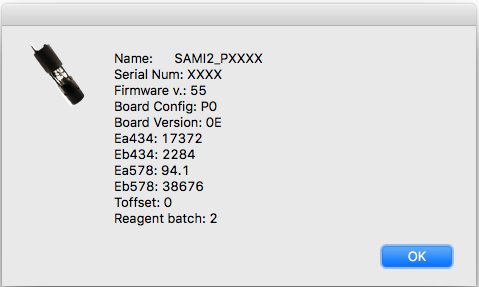
\includegraphics[width=0.6\textwidth]{figs/Cal_Info.png}
    \caption{Read calibration window.}
    \label{fig:CalInfo}
    \end{figure}
    
    \item[] \textbf{Read Cal Info:} Figure \ref{fig:CalInfo} lets you view E values, \instType{} temperature offset compared to NIST-traceable standard, and reagent type (1 is un-purified; 2 is purified). These values should match the values on the calibration certificate that was shipped with the \instType{} after the most recent refurbishment.  If values do not match, contact Sunburst Sensors before deployment.
\end{itemize}


\subsubsection{Help Menu}

Various documents are available via the Help menu, including this manual, release notes for the software detailing what changes have been made, use of external instruments, etc.

\begin{itemize}
    \item[] \textbf{View Sunburst Website:}
    This heading will direct you to \url{http://www.sunburstsensors.com} for convenient access to our business, research, and contact information. 
    
    \item[] \textbf{Send us Email:}
    Directs email to Info@sunburstsensors.com
    
    \item[] \textbf{About SAMI application (PC):}
    Brings up an information and credits window.
    
    \item[] \textbf{Check for Updates:}
    If you have an internet connection the \instType{} Client software will automatically check the Sunburst Sensors website for updates to the software upon launch. You can manually check via this menu item.
\end{itemize}


\subsubsection{Control Tab}

The \textbf{Control} tab is where you establish communication and power with the \instType{}, start and stop sample collection, and download data.

\begin{figure}[ht]
\centering
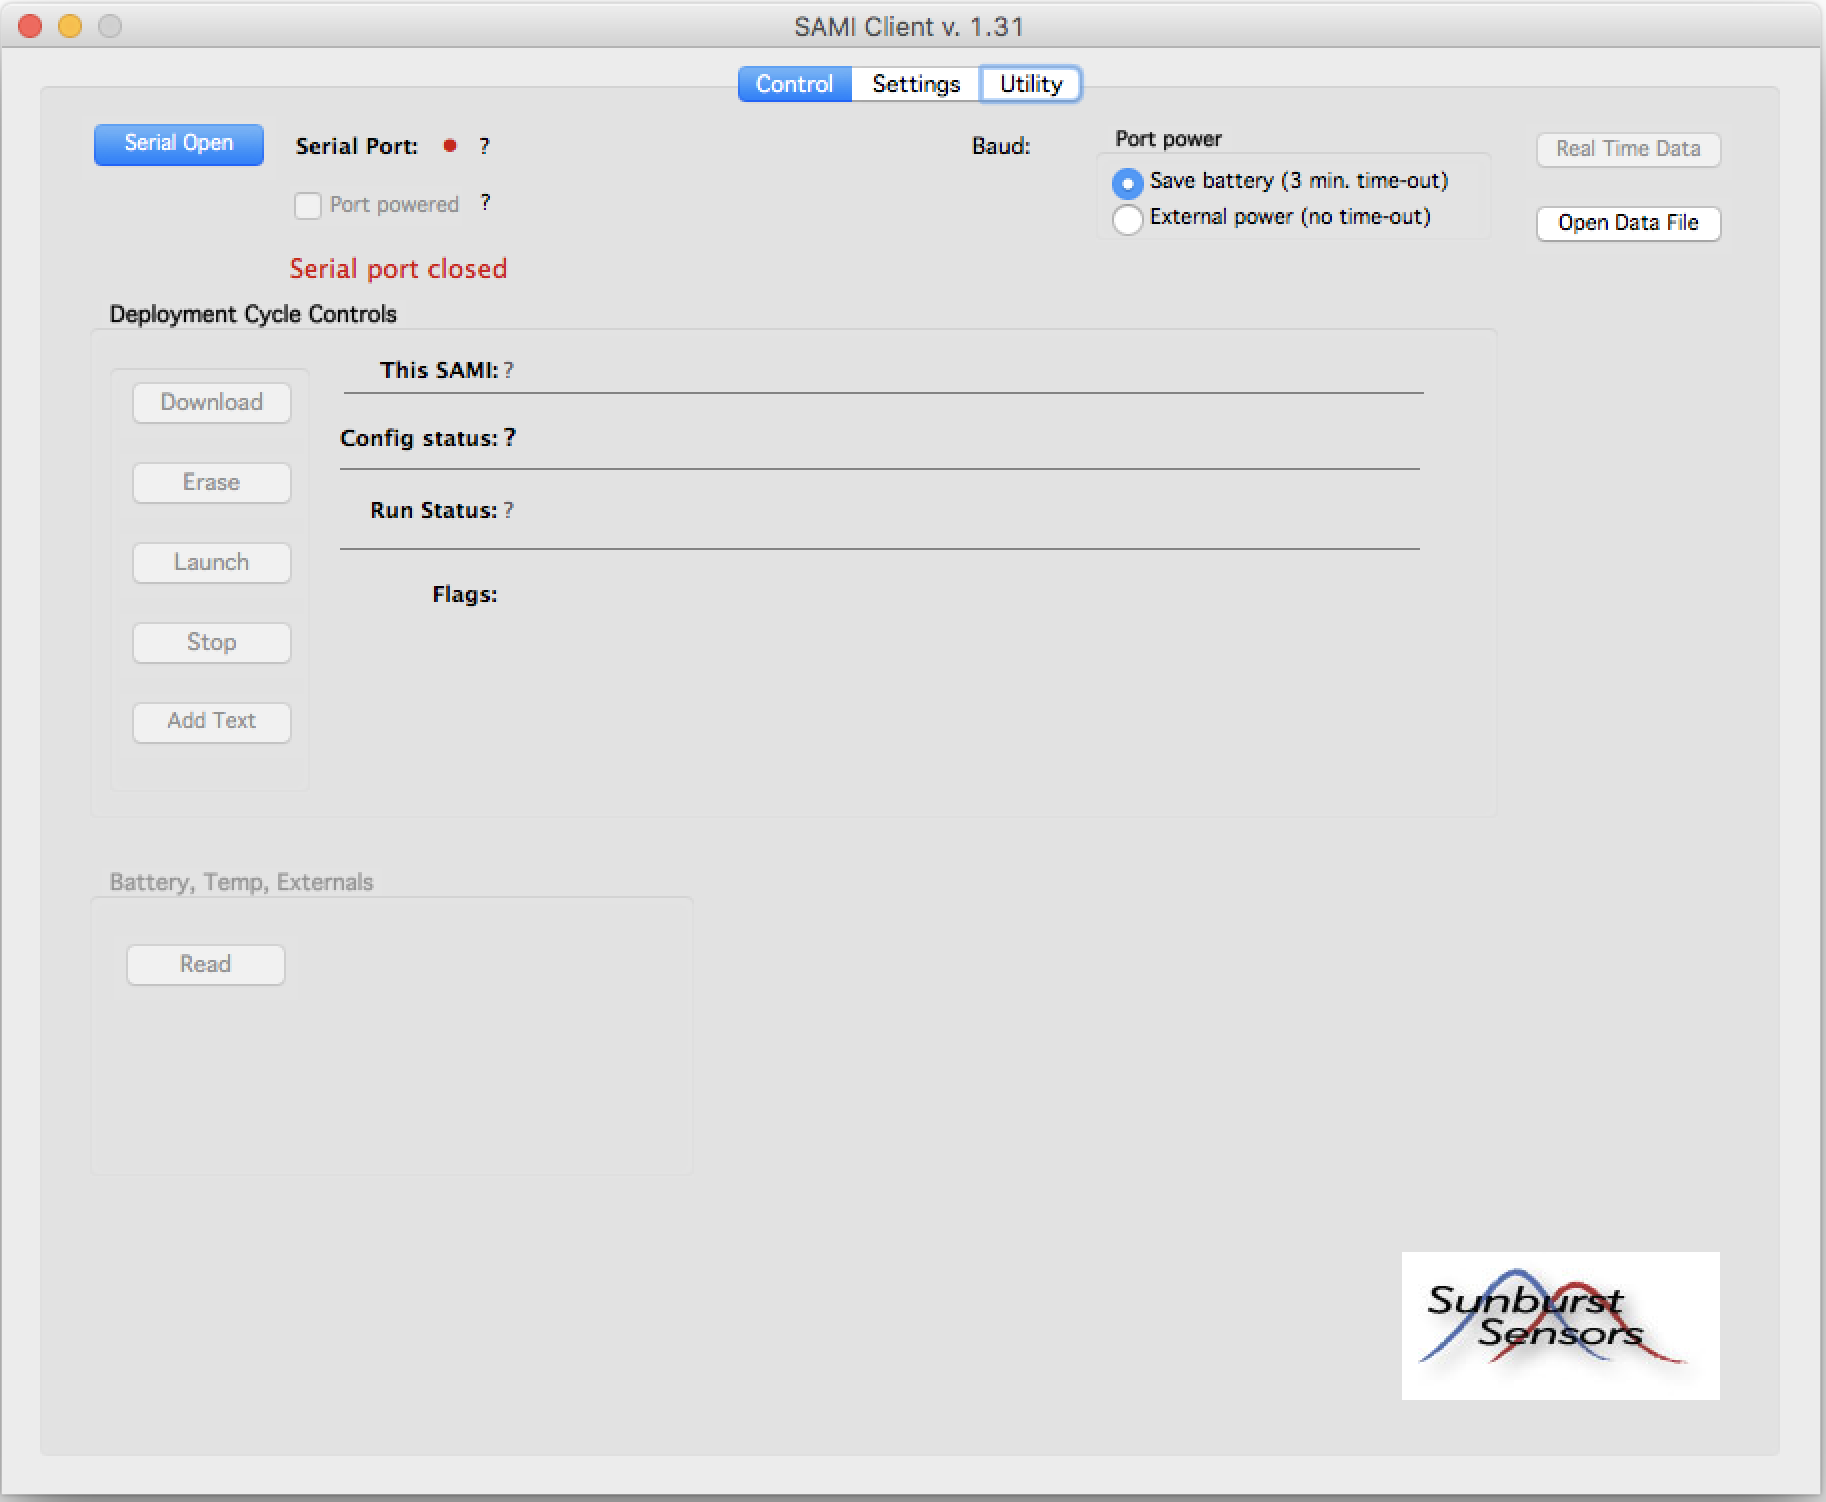
\includegraphics[width=1.0\textwidth]{figs/Cntl_Tab.png}
\caption{Control tab.}
\label{fig:CntlTab}
\end{figure}


\subsubsection{Serial Communication}
\label{Serial}

The \textbf{Serial Open/Serial Close} button engages \textbf{SAMI\_Client} to communicate with your instrument. To establish communication, attach the communication cable to your computer and \ifcase \inst {\instType{}, and power to 12\,V supply or battery.} \or {\instType{}.} \or {and power \instType{}.} \fi In Edit $\rightarrow$ Preferences (PC), or SAMI Client $\rightarrow$ Preferences (Mac) select the appropriate serial port. Click the \textbf{Serial Open} button to begin communication with your \instType{}. The indicator next to the Serial Port text will specify if your \instType{} is interfaced with your computer. A red dot indicates a closed serial port while a green dot indicates an open serial port (Figures \ref{fig:InstInterface} and \ref{fig:CntlTab}). 

If the \textbf{Auto-Open Serial } box is checked in the \textbf{Preferences} pop-up page, the \textbf{Serial Open/Serial Close} button will no longer be visible and the \instType{} will automatically try to establish communication when it is powered on.

\begin{figure}[ht]
\centering
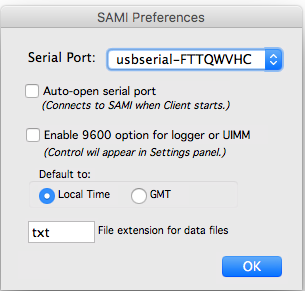
\includegraphics[width=0.5\textwidth]{figs/Prefs.png}
\caption{Communication preferences pop-up window}
\label{fig:Prefs}
\end{figure}


\subsubsection{Power Settings}
\label{sec:SoftwarePower}

\begin{itemize}
    \item[] \textbf{Port Powered/Re-power:}
    You can communicate with the \instType{} and program it for deployment without connecting to external power.  To conserve the small internal battery, the  communications will time out after 3 minutes, unless you override this feature by selecting the \textbf{External Power} radio button. If the port does time out, you can re-open it by simply clicking the \textbf{Re-power} check box. If communications has timed-out, you cannot send commands or program the \instType{} until the port is re-powered.
    
    If the \instType{} is \ifcase \inst {running (while connected to 12\,V power),} \else {running,} \fi however, the  will send data out over the serial port after each measurement or other event, even if the port is timed out (The \instType{} powers up the port just long enough to send data).
    
    \item[] \textbf{Save Battery:}
    The Save battery option should be selected when not connected to external power. This allows the \instType{} to go into time-out after three minutes and preserves the internal battery. This function may also be controlled from the \textbf{Utility} tab.
    
    \item[] \textbf{External power:}
    If the \instType{} is connected to a 12\,VDC power supply, you can select this option to keep communication open with the \instType{} Client at all times. If \textbf{External Power} is selected, the message \say{Port power on until disconnected} will appear under serial port. This function may also be controlled from the utility tab.
\end{itemize}


\subsubsection{Deployment Cycles Controls Panel} 

\begin{itemize}
    \item[] \textbf{Download}
    The \textbf{Download} button will copy data stored on your \instType{} to a location you select on your computer.  A default file name of \verb|SAMI_UnitName_DDMMYY| will be suggested in the save dialog. Data will not be erased from the \instType{} by using the Download function.  If download fails, try it again.
    
    \item[] \textbf{Erase:}
    The \textbf{Erase} button will clear the memory on the \instType{} of the data that it previously collected. To launch your \instType{} you must erase all data stored on the \instType{}. If you wish to save the data from your last data collection you MUST download the information before it is erased. If you attempt to erase data before it has been downloaded, you will get a warning message \say{Data has not been downloaded!} \textbf{OK} will erase all data and settings! 
    
    \item[] \textbf{Add Text:}
    The \textbf{Add Text} button allows you to add notes to the instruments memory. The notes will be displayed in the data output files and can be accessed from the Toolbar SAMI $\rightarrow$ Read SAMI Text.  
    
    \item[] \textbf{Launch}
    \label{Launch:}
    Unless the \instType{} has been erased, it cannot be launched. Prior to launch, use the controls in the Settings Tab to configure the \instType{}; setting the start time, sample interval, etc.  
    If you have set a launch time that has passed, you will get the message \say{Start is less than 10 seconds from now!  Would you like to start in 10 seconds?}. This may be OK for bench-top testing, but if you require data aligned to the hour, you should program the start time accordingly.
           
    \item[] \textbf{Stop:}
    The \textbf{Stop} button will end the launch of your instrument and sampling will cease. Data will be saved in the memory of your instrument.
\end{itemize}


\subsubsection{Configuration status Panel} 

\begin{itemize}
    \item[] \textbf{Serial Port Opened:}
    \label{Serial}
    The \instType{} has established communication with your computer. 
    
    \item[] \textbf{Config loaded and \instType{} started:}
    Indicates that your program has launched and measurement collection has begun.
    
    \item[] \textbf{(\#:) of Pages downloaded}
    This message appears when a measurement sequence has been stopped and you have downloaded a file. 
    
    \item[] \textbf{Erased:}
    The memory has been cleared and you may begin another measurement sequence.
\end{itemize}


\subsubsection{Flags}

The Flags section will display messages that indicate status:
 
This \instType{}: \quad Name: \quad SN: \quad Hardware: \quad Firmware:

\begin{itemize}
    \item[] \textbf{Recording Started:}
    Data is being collected and stored in your instrument's memory.
    
    \item[] \textbf{Recording Stopped:}
    The measurement sequence has stopped. The data has not yet been downloaded or erased.
    
    \item[] \textbf{Downloaded:}
    The measurement sequence has been stopped.  The data has been downloaded, but not erased. Erase your data before continuing with another sequence of measurements.   
    
    \item[] \textbf{Run Status:}
    
    While the program is running, the Run Status will display the date, time, number of data files collected, and the memory used. The Run Status section will remain blank if the program is not running, the files have been downloaded, or the data file is erased.
\end{itemize}


\subsubsection{Battery, Temp, Externals Panel}

\begin{wrapfigure}[4]{r}{0.6\textwidth}
\centering
\vspace{-5mm}
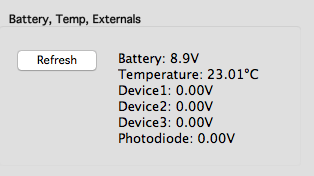
\includegraphics[width=0.8\textwidth]{figs/Read_Batt.png}
\caption{Battery, Temperature, Externals panel}
\label{fig:ReadBatt}
\end{wrapfigure}

Clicking the \textbf{Read} button updates information on the battery voltage, the temperature in Celsius, and the output voltage of any external devices.

\vspace{30mm}


\subsubsection{Settings Tab}

\paragraph{Overview}
The \textbf{Settings} tab contains the various control panels used to configure the instrument prior to a deployment. These control panels allow the user to set the start time and run duration, sampling interval, etc. It is important to note that these settings are not sent to the instrument until the user launches the unit via the \textbf{Launch} button in the deployment controls (section \ref{Launch}).  

\begin{figure}[h]
\centering
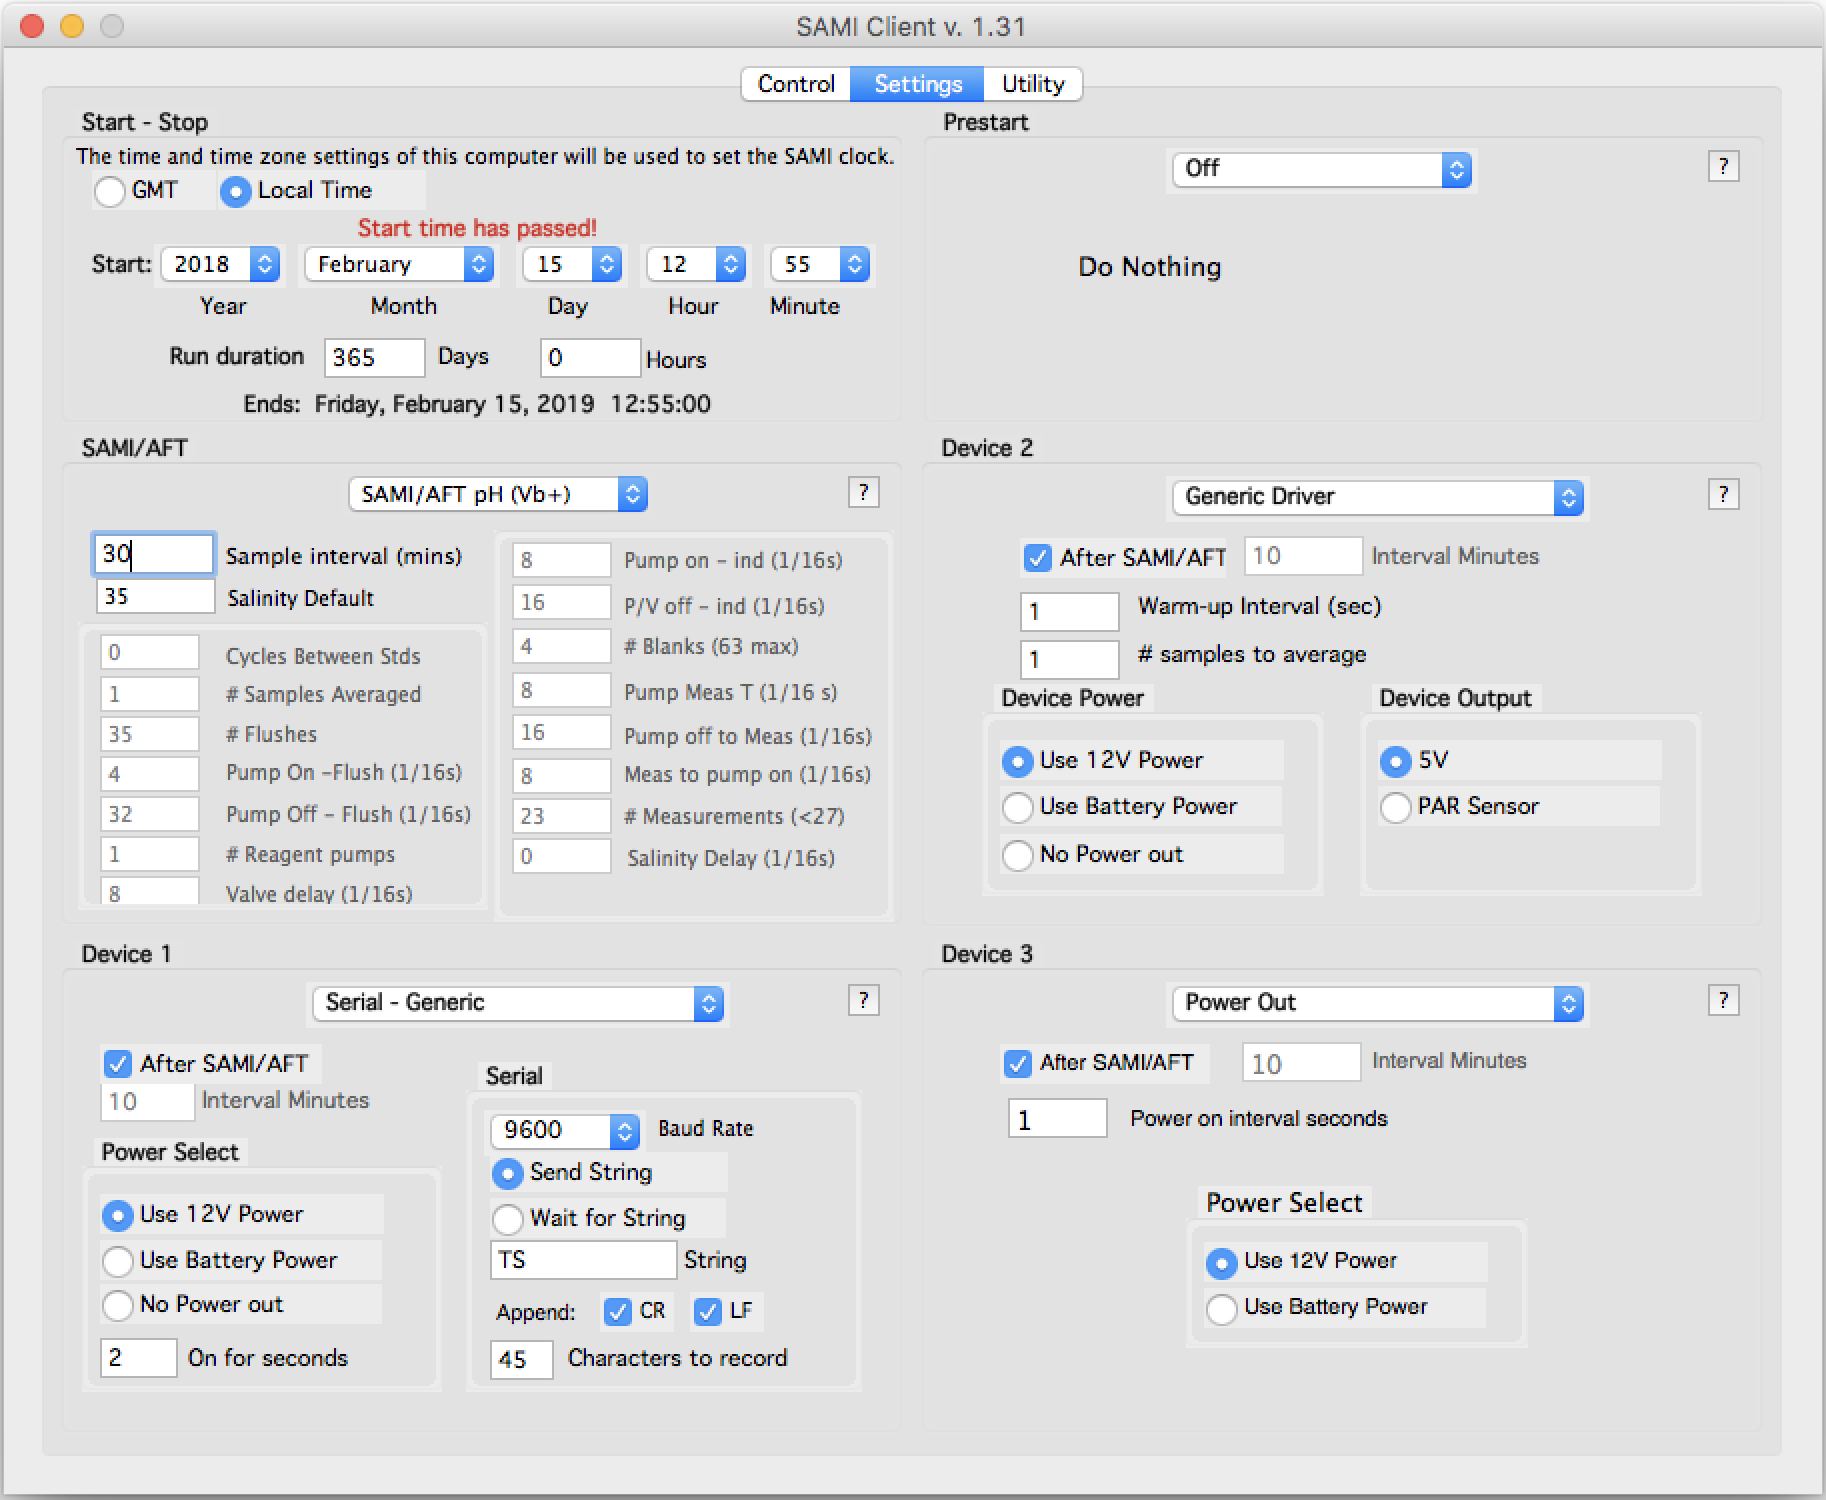
\includegraphics[width=1.0\textwidth]{figs/Set_Tab2.png}
\caption{Settings tab.}
\label{fig:SetTab2}
\end{figure}


\subsubsection{Start-Stop Panel}

In the \textbf{Start-Stop} panel in the upper left hand corner of the \textbf{Settings} tab you will enter your deployment start time and the run duration. You may enter the exact time you wish to launch your instrument, accurate to five minutes. Note that you may display your time in GMT or local time. However, \textbf{data is stored on the \instType{} in GMT, regardless of the time format set here.} When you enter the run duration in the specified box, a message appears below which will calculate the end time and date. 

In the event that the start time has passed, you will receive a message informing you the start time has passed. When you Launch your instrument a message box will ask if you wish to begin sampling in ten seconds.  By selecting \textbf{OK} measurements will begin immediately. Otherwise you may select a new start time by selecting \textbf{Cancel}.


\subsubsection{SAMI/AFT Panel}

The \textbf{SAMI/AFT} panel is where you will enter the sampling interval. In the dropdown menu in the top center of the box, select \textbf{SAMI-pH (Vb+)}. The sample interval must be entered in minutes and with a time of no less than five minutes (15\,min is optimal).  Enter the approximate or measured salinity of the sample in \textbf{Salinity Default}.  This salinity will be used to calculate \pKa for the pH measurement.  The grayed-out controls on the right hand side of the control panel are not user adjustable, but visible for trouble shooting and support.


\subsubsection{External Device Panels}

\ifcase \inst	%iSAMI

External devices are not supported by the \instType{}.

\else			%SAMI/AFT

The \instType{} supports up to three external devices, such as PAR sensors, fluorimeters, dissolved oxygen optode, or similar. It can read and log device output. It will support one RS232 serial device and two 0--5\,VDC output devices, or three 0--5\,VDC devices with no serial device. These devices can be scheduled with reference to the \instType{}'s own measurements, occurring immediately after the measurement has completed, or on a set interval.

Contact Sunburst if you wish to control an external device with the \instType{}. The \instType{} is not configured to support external devices in the base model (there is no wiring to support the externals).

\paragraph{Generic Driver}
The generic driver supports 0--5\,VDC input. Select the scheduling of the device by specifying whether to activate after the \instType{} measurement or at a fixed interval. The \textbf{Warm-Up Interval} allows the external device to stabilize before measuring and should be set in accordance with manufacturers suggestions. The \textbf{\# samples to average} allows multiple readings to be averaged. The power selection allows devices that have their own power conditioning to access the instrument batteries directly and thereby increase efficiency.  Some devices, such as a PAR sensor, require no power.  Other options include generic serial, serial, devices, etc.

\fi


\subsubsection{Utility Tab}

\begin{figure}[ht]
\centering
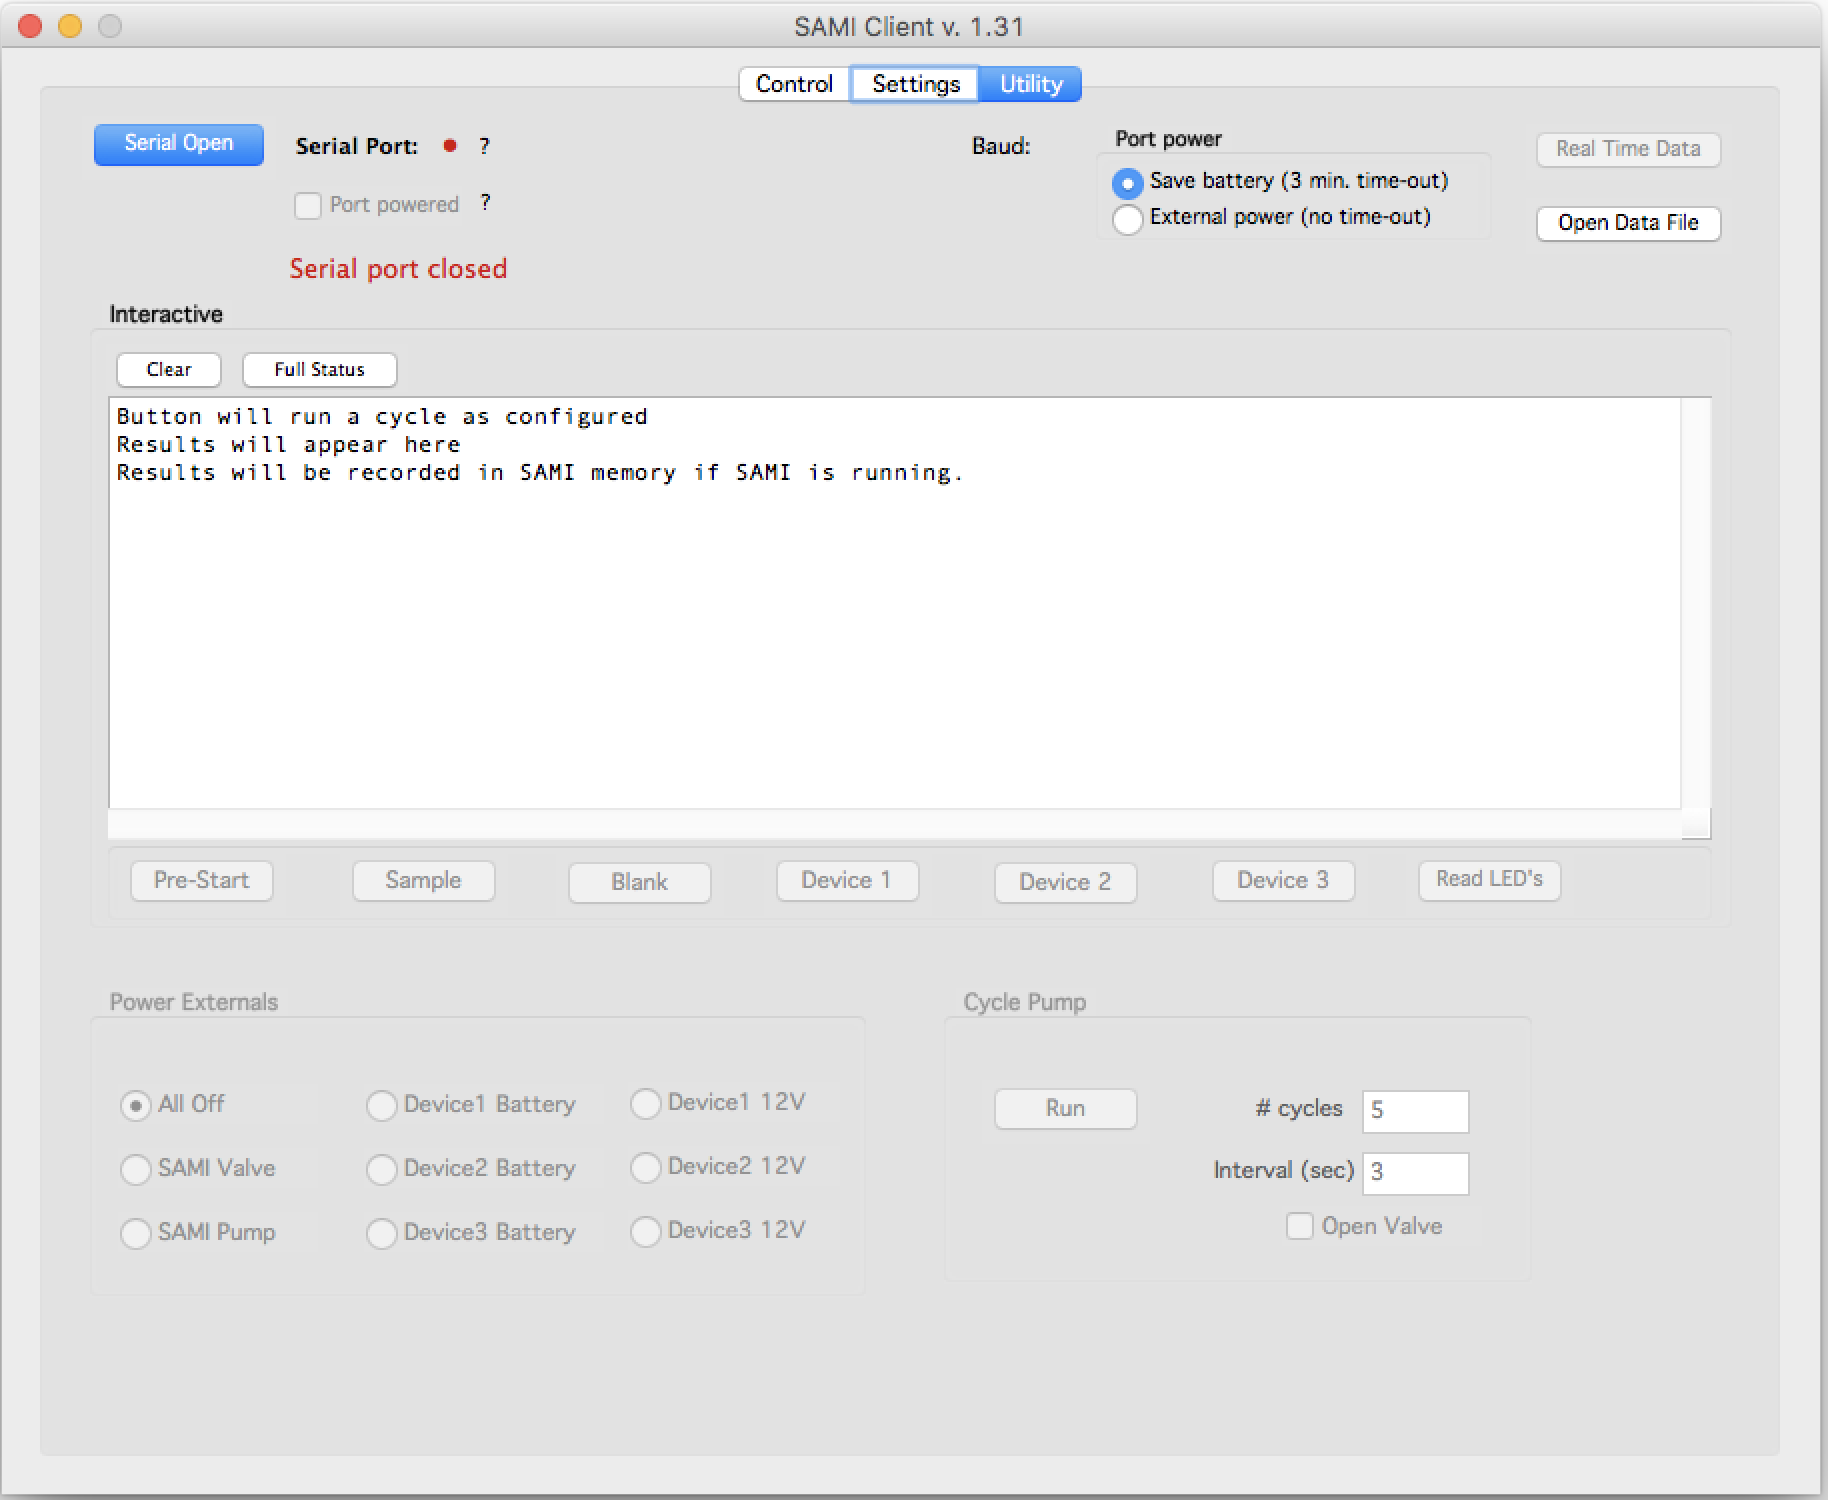
\includegraphics[width=1.0\textwidth]{figs/Util_Tab.png}
\caption{Utility tab.}
\label{fig:UtilTab}
\end{figure}

The \textbf{Utility} tab is generally used for trouble-shooting, to flush the \instType{} prior to storage or at the end of a deployment, and for data processing.


\subsubsection{Serial Port Open-Close, Port Power}

These functions can be controlled from the \textbf{Control} tab or from the \textbf{Utility} tab. See explanation of their functions in section \ref{Serial}.


\subsubsection{Interactive}

\ifcase \inst	%iSAMI

The \textbf{Interactive} panel will give you live feed on the data that your instrument is collecting when the communication cable is connected to 12\,V power. With each measurement, a string of information is written to the window. The first line will start with \say{Launch.} The next line will have the headers for the following columns of data: sample type, yearday, initial internal temperature, $\textrm{(434\,nm reference, 434\,nm signal, \linebreak 578\,nm reference, 578\,nm signal)}_n$, final internal temperature, battery voltage, external temperature. All readings are 14-bit. $n$ is \# Blanks plus \# Measurements from the Settings; default is 27. Data will be written to the screen each time a measurement is taken. This information is mostly for trouble-shooting. The records are not processed (i.e. pH, etc. is not calculated). At the top of the display you will notice a button marked \textbf{Clear} which will clear the display. The \textbf{Clear} button will not erase data from the memory.

\or			%SAMI/AFT

The \textbf{Interactive} panel will give you live feed on the data that your instrument is collecting. With each measurement, a string of information is written to the window. The first line will start with \say{Launch.} The next line will have the headers for the following columns of data: sample type, yearday, initial internal temperature, $\textrm{(434\,nm reference, 434\,nm signal, \linebreak 578\,nm reference, 578\,nm signal)}_n$, final internal temperature, battery voltage, external temperature. All readings are 12-bit. $n$ is \# Blanks plus \# Measurements from the Settings; default is 27. Data will be written to the screen each time a measurement is taken. This information is mostly for trouble-shooting. The records are not processed (i.e. pH, etc. is not calculated). At the top of the display you will notice a button marked \textbf{Clear} which will clear the display. The \textbf{Clear} button will not erase data from the memory.

\fi

\begin{itemize}
    \item[] \textbf{Read LEDs:}
    The \textbf{Read LEDs} button allows the user to check the Reference and Signal intensities of the instrument.  This can help alert the user to problems such as a blocked flow cell path or malfunctioning valve and can otherwise help to ensure the instrument is ready to deploy.
    
    \item[] \textbf{Pre-Start:}
    The instrument can be programmed to perform functions while it is waiting to start.  If this has been configured, it will read battery and temperature as programmed in the Pre-start section of the \textbf{Control} tab.
    
    \item[] \textbf{Sample:}
    The \textbf{Sample} button will run a measurement according to your programmed specifications. The measurement will not be saved in your stored data but will display in the \textbf{Interactive} panel unless the instrument has been launched.
    
    \item[] \textbf{Device 1, 2, 3:}
    \ifcase \inst	%iSAMI
    
    External devices are not supported by the \instType{}.
    
    \or			%SAMI/AFT

    This will take a reading of the device selected.  The data will not be saved in your stored data but will display in the \textbf{Interactive} panel.
    
    \fi
\end{itemize}


\subsubsection{Power Externals}

\ifcase \inst	%iSAMI

The \textbf{Power External} buttons located beneath the Interactive screen and can power the pump or valve, or an external device using 12\,VDC or battery voltage. External devices are not supported by the \instType{}. 

\or			%SAMI

The \textbf{Power External} buttons located beneath the Interactive screen and can power the pump or valve, or an external device using 12\,VDC or battery voltage.  This is useful for testing and running a CTD that is powered by the \instType{}.

\or			%AFT

The \textbf{Power External} buttons located beneath the Interactive screen and can power the pump or valve, or an external device using 12\,VDC.  This is useful for testing and running a TSG that is powered by the \instType{}.

\fi


\subsubsection{Cycle Pump}

The \textbf{Cycle Pump} function is available to flush your instrument. Flushing is an important function for the health of your \instType{} as well as to maintain a clear optical path. To flush the pH \instType{} you will need to attach the small fluid bag that came with the \instType{} or submerge the inlet tubing in deionized water, and click on \textbf{pH Flush}. The instrument will need to be flushed after each deployment in seawater.  \textit{Do not} check the \textbf{Open Valve} box, as this will flush the instrument with reagent.

The \textbf{Open Valve} box will initiate the valve during the pumping cycle. By checking this box, the initiation of the valve will pump reagent in your \instType{}-pH. The \textbf{\# cycles} refers to the number of \ifcase \inst {25\,$\mathrm{\mu L}$} \else {50\,$\mathrm{\mu L}$} \fi pumps you wish to flush through the instrument. You may choose up to 99. \textbf{Interval (secs)} refers to the amount of time between each \ifcase \inst {25\,$\mathrm{\mu L}$ pump (1\,s or greater).} \else {50\,$\mathrm{\mu L}$ pump (1\,s or greater).} \fi


\subsection{Viewing Data}

\ifcase \inst	%iSAMI

Data can be viewed in real time or imported from a file after download. On the \textbf{Control} or \textbf{Utility} tab the \textbf{Read Real Time} button becomes activated when the software detects a new measurement record (if you have connected to a \instType{} that is already running) or immediately after the \textbf{Launch} button is pushed. Data that has been previously downloaded can be imported by selecting the \textbf{Open Data File} button or selecting \textbf{Import Data File} from the File menu. The \instType{} must be powered with a 12\,VDC supply in order to view realtime data.

\else			%SAMI/AFT

Data can be viewed in real time or imported from a file after download. On the \textbf{Control} or \textbf{Utility} tab the \textbf{Read Real Time} button becomes activated when the software detects a new measurement record (if you have connected to a \instType{} that is already running) or immediately after the \textbf{Launch} button is pushed. Data that has been previously downloaded can be imported by selecting the \textbf{Open Data File} button or selecting \textbf{Import Data File} from the File menu.

\fi

\begin{itemize}
    \item[] \textbf{Data Overview:}
    Raw \instType{} data is stored as records while the \instType{} is running. These same records are transmitted over the serial port as well, so the client software will recognize and interpret them in real time.
    
    \item[] \textbf{Raw Record Structure:}
    There are two main types of records recorded by the instrument. There are data records and information records.  Every record leads with an identifying number (Record Type) and a 4-byte time stamp. Information records note events such as start, stop, low battery and possible errors if one should occur. Data records follow the type/time fields with a series of fields composed of the various readings (e.g. temperature, dark signal) needed for the measurement.  In raw format these readings are not especially informative except in trouble-shooting situations.
    
    \item[] \textbf{Computed fields:}

    \ifcase \inst	%iSAMI
    
    Computed fields consist of data derived from the raw records. For example, the raw thermistor reading is stored as a 14-bit number (0--16384). The temperature field is the temperature calculated from that raw number. Time is stored as a 4-byte number reflecting total seconds since Jan 1, 1904, while calculated fields allow time to be displayed in a variety of formats.
    
    \else		%SAMI/AFT
    
        Computed fields consist of data derived from the raw records. For example, the raw thermistor reading is stored as a 12-bit number (0--4095). The temperature field is the temperature calculated from that raw number. Time is stored as a 4-byte number reflecting total seconds since Jan 1, 1904, while calculated fields allow time to be displayed in a variety of formats.
    
    \fi
    
    \item[] \textbf{Viewing real time data:}
    
    \ifcase \inst	%iSAMI
    
     The \textbf{Real Time Data} button plots data that is being collected by the instrument in real time. When you click on the \textbf{Real Time Data} button, a pop-up with a drop down menu titled Column Set will appear. \instType{} Client has a number of previously compiled parameter sets that you can choose from in Column Set Lists. Choose \textbf{pH$\_$ConstSal}. Be sure that the approximate salinity is entered in \textbf{Salinity Default} on the \textbf{Settings} tab. A new window will open with data in spreadsheet format. A drop down menu titled Display Type allows you to view data in spreadsheet or scatter plot format.

    \or			%SAMI
    
      The \textbf{Real Time Data} button plots data that is being collected by the instrument in real time. When you click on the \textbf{Real Time Data} button, a pop-up with a drop down menu titled Column Set will appear. \instType{} Client has a number of previously compiled parameter sets that you can choose from in Column Set Lists. Choose \textbf{pH$\_$ConstSal} if you did not measure salinity with a CTD that was controlled by the \instType{}.  Be sure that the approximate salinity is entered in \textbf{Salinity Default} on the \textbf{Settings} tab.  Choose \textbf{pH$\_$MeasSal} if the \instType{} logged data from a CTD. Select \textbf{Make View Win} to view the data. A new window will open with data in spreadsheet format. A drop down menu titled Display Type allows you to view data in spreadsheet or scatter plot format.

    \or			%AFT
      The \textbf{Real Time Data} button plots data that is being collected by the instrument in real time. When you click on the \textbf{Real Time Data} button, a pop-up with a drop down menu titled Column Set will appear. \instType{} Client has a number of previously compiled parameter sets that you can choose from in Column Set Lists. Choose \textbf{pH$\_$ConstSal} if you did not measure salinity with a TSG that was controlled by the \instType{}.  Be sure that the approximate salinity is entered in \textbf{Salinity Default} on the \textbf{Settings} tab.  Choose \textbf{pH$\_$MeasSal} if the \instType{} logged data from a TSG. Select \textbf{Make View Win} to view the data. A new window will open with data in spreadsheet format. A drop down menu titled Display Type allows you to view data in spreadsheet or scatter plot format.
    
    \fi
    
    \begin{figure}[!h]
    \centering
    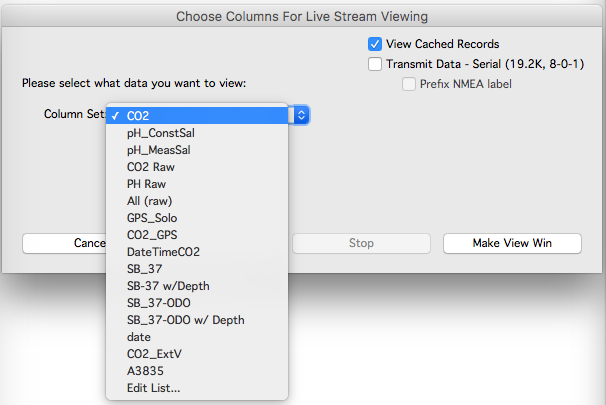
\includegraphics[width=0.5\textwidth]{figs/Real_Time.png}
    \caption{Real-time data dropdown menu.}
    \label{RealTime}
    \end{figure}
    
    \item[] \textbf{Spreadsheet:}
    The Spreadsheet format will allow you to view the data being collected as a list (Figure \ref{fig:ProcData}). 
    \vspace{5mm}
    
    \begin{figure}[!h]
    \centering
    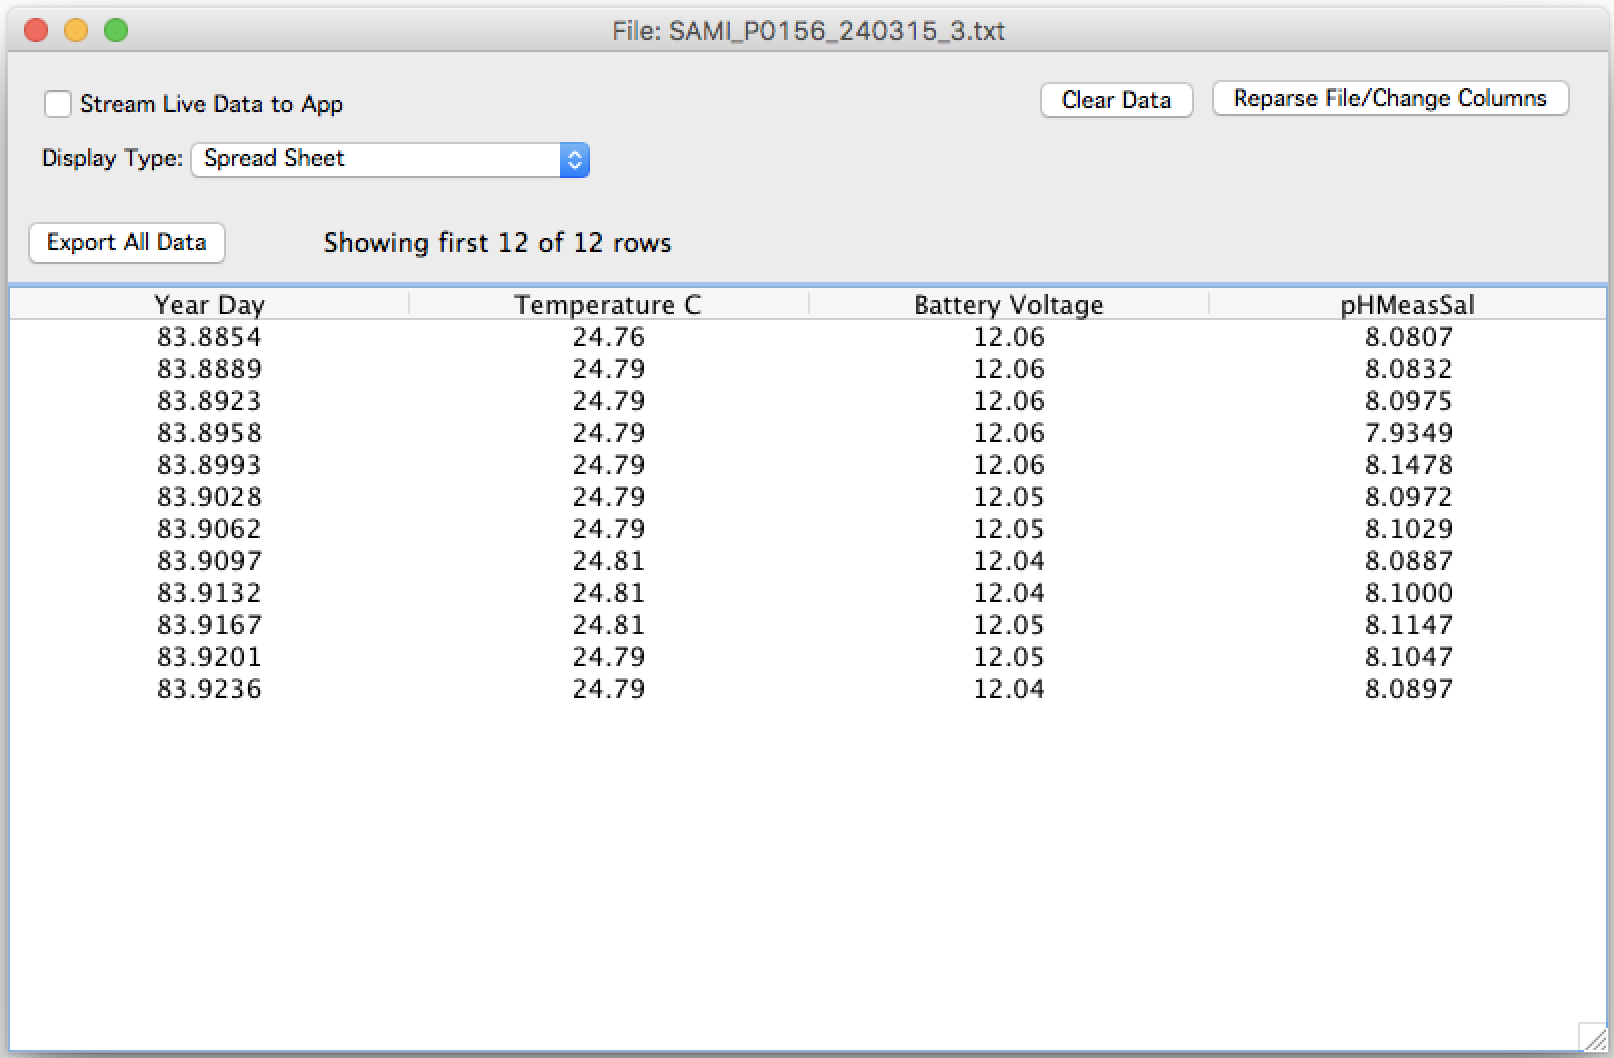
\includegraphics[width=0.7\textwidth]{figs/Proc_Data.png}
    \caption{Processed data in spreadsheet format.}
    \label{fig:ProcData}
    \end{figure}
    
    \item[] \textbf{Scatter Plot:}
    Under the Scatter Plot data display select the x-axis and y-axis parameters you wish to plot (Figure \ref{fig:PlotData}). 
    
    \begin{figure}[!h]
    \centering
    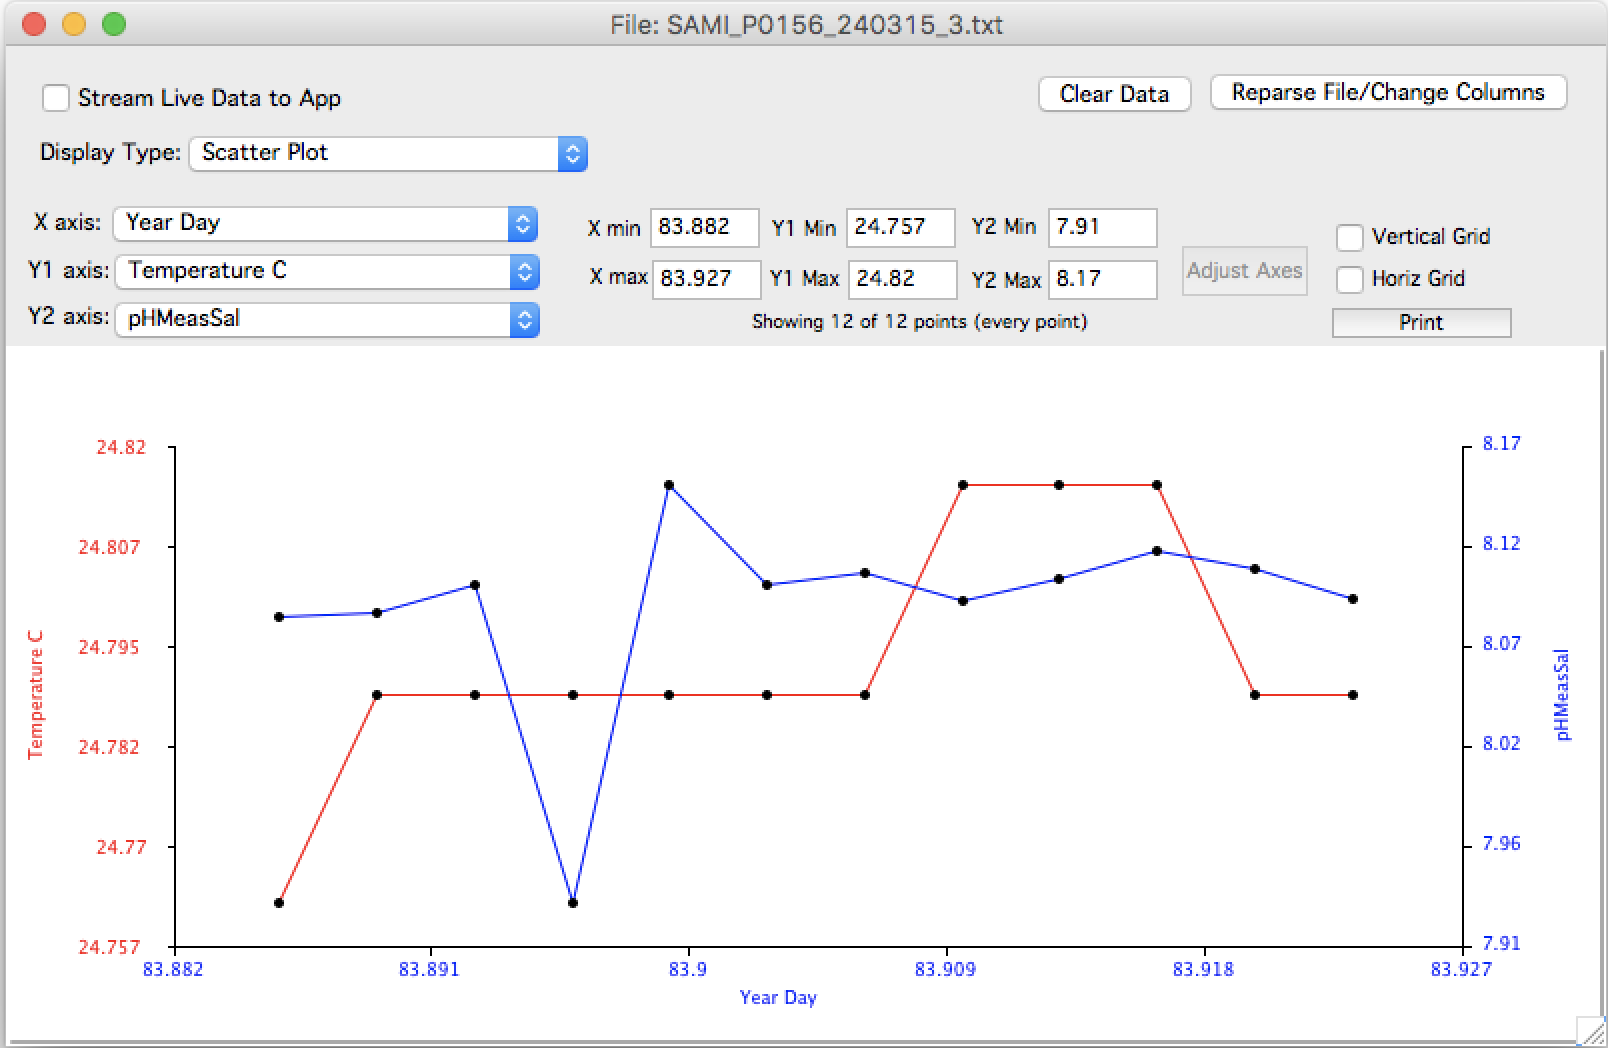
\includegraphics[width=0.7\textwidth]{figs/Plot_Data.png}
    \caption{Processed data in scatter plot format.}
    \label{fig:PlotData}
    \end{figure}
    
    \item[] \textbf{Creating your own set of parameters to view:}
    If a pre-fabricated set of parameters does not include the information that you would like to view, you may create and name your customized Column Set List. By selecting \textbf{Edit List...} from the Column Set drop-down window you will receive a Set List Editor. You may adapt a previously existing list or create a new one. 
    
    Editing a pre-existing list is done by highlighting the list you wish to edit and clicking the button in the lower right hand corner labeled \textbf{Edit}. A list of the parameters appears in a new window. The left side window labeled Columns will display all parameters contained in the Column Set List. Clicking the \textbf{Add} button below the window will make available two drop down menus on the right side of the window. The \textbf{Column Type} drop-down menu will provide you with the classifications of parameter we have to choose from. You may be interested in viewing raw data or processed data. By selecting the type of data you can choose the exact parameter you wish to plot in the Column Name drop-down menu below. There you may select from a number of different parameters to populate your Column Set List: sample or reference signals of a specific wavelength, ratio of signals to reference, temperature, time, battery voltage, and pH. 
    
    To create your own Column Set List, return to the Column Set List editor. Select \textbf{Add} from the buttons at the bottom of the window. A Column Editor will appear with an untitled Column Set List. Name your Set List and populate the parameters in the same fashion as described above.  
\end{itemize}


\subsection{Data Processing}

\subsubsection{Processing text files}

\ifcase \inst	%iSAMI

Once data has been downloaded, you can view raw and processed data with \instType{} Client software. Go to File menu and select \textbf{Open Data File}. A window will appear that asks you to select what data you want to extract from the file. In the drop down menu, select \textbf{pH\_ConstSal} for constant salinity (the approximate salinity of your sample must be entered in the \textbf{Salinity Default} box on the \textbf{Settings} tab). If you independently measured CTD data and want to use the measured salinity to calculated the pH, you will need to process the data using QC\_PH, as described in section \ref{sec:RunQC_PH}.

\or			%SAMI

Once data has been downloaded, you can view raw and processed data with \instType{} Client software. Go to File menu and select \textbf{Open Data File}. A window will appear that asks you to select what data you want to extract from the file. In the drop down menu, select \textbf{pH\_ConstSal} for constant salinity (the approximate salinity of your sample must be entered in the \textbf{Salinity Default} box on the \textbf{Settings} tab).  If you logged CTD data with the \instType{}, select \textbf{pH\_MeasSal}. If you logged CTD data independently and want to use the measured salinity, you will need to process the data using QC\_PH, as described in section \ref{sec:RunQC_PH}.

\or			%AFT

Once data has been downloaded, you can view raw and processed data with \instType{} Client software. Go to File menu and select \textbf{Open Data File}. A window will appear that asks you to select what data you want to extract from the file. In the drop down menu, select \textbf{pH\_ConstSal} for constant salinity (the approximate salinity of your sample must be entered in the \textbf{Salinity Default} box on the \textbf{Settings} tab).  If you logged TSG data with the \instType{}, select \textbf{pH\_MeasSal}. If you logged TSG data independently and want to use the measured salinity, you will need to process the data using QC\_PH, as described in section \ref{sec:RunQC_PH}.

\fi

Next, click on the \textbf{Parse File} button. Data can be viewed as a spreadsheet or Scatter Plot and exported as a text file. Although you can only view the first 500 rows of data, you can process and export the entire data file. Note that this is preliminary data.  A standalone Matlab program, included on your disc, filters and processes the data more thoroughly.  This is described in section \ref{sec:QC_PH}.


\subsubsection{Processing hex files from a custom interface}

The \instType{} data can be collected from the user's system via RS-232.  Data collected this way will be in hex format.  A hex file can be imported and processed in SAMI\_Client. From the \textbf{File} menu select \textbf{Import hex File.}  In the dropdown menu choose \textbf{pH\_const sal}. In the upper right hand corner of the Import menu, select \textbf{Choose Config File} and choose a configuration file.  A configuration file is saved when you launch the \instType{}. A generic configuration file can be saved at any time.  Once the hex data is imported, the functions of the program are the same as when reading \instType{} txt files.